\documentclass[10pt]{article}
\usepackage[latin1]{inputenc}
\usepackage{amsmath}
\usepackage{amsfonts}
\usepackage{amssymb}
\usepackage{graphicx}
\graphicspath{{./img/}}
\usepackage{textcomp}
\usepackage{siunitx}
\usepackage[a4paper,margin=3cm]{geometry}
\usepackage{multirow}
\title{Modelling}
\author{NTNU - iGem Team 2016}



\begin{document}
\maketitle

\begin{center}
\section*{Abstract}
The following is the documentation and analysis from the modelling of a \textit{XOR} logic gate. This task included a formulation of the model by studying the operating principle of the gate. An expected response function was proposed accordingly. The model was solved in both dynamic state and steady state for a range of inputs for an initial set of kinetic parameters. The model was improved by modifying some equilibrium constants in a given range. An improved response surface was obtained as a result. 
\end{center}

\section{Model set up}

\subsection{Gate operation principle}
The system we are going to model is a \textit{XOR} gate. The behaviour for this gate is shown on Table \ref{tb:xor}. 
\begin{table}[h]
	\centering
	\caption{XOR gate table} \label{tb:xor}
	\begin{tabular}{c|c|c}
	\multicolumn{2}{c|}{Input} & Output \\ \hline
	A & B & A~\textit{XOR}~B\\ 
	0 & 0 & 0 \\
	1 & 0 & 1 \\
	0 & 1 & 1 \\
	1 & 1 & 0 
	\end{tabular}
\end{table} \par  
However, in biological systems the inputs and outputs are not discrete values. The expected behaviour in a continuous system cannot be simplified to a table. For this purpose an ideal function has been defined:
\begin{equation}
z = x^2 + y^2-2xy
\end{equation} 
where \textit{x} and \textit{y} are the inputs and \textit{z} is the output.\\
Figure \ref{fig:ideal} illustrates the behaviour of this function for values of the inputs between 0 and 1. 
\begin{figure}[h]
	\centering
	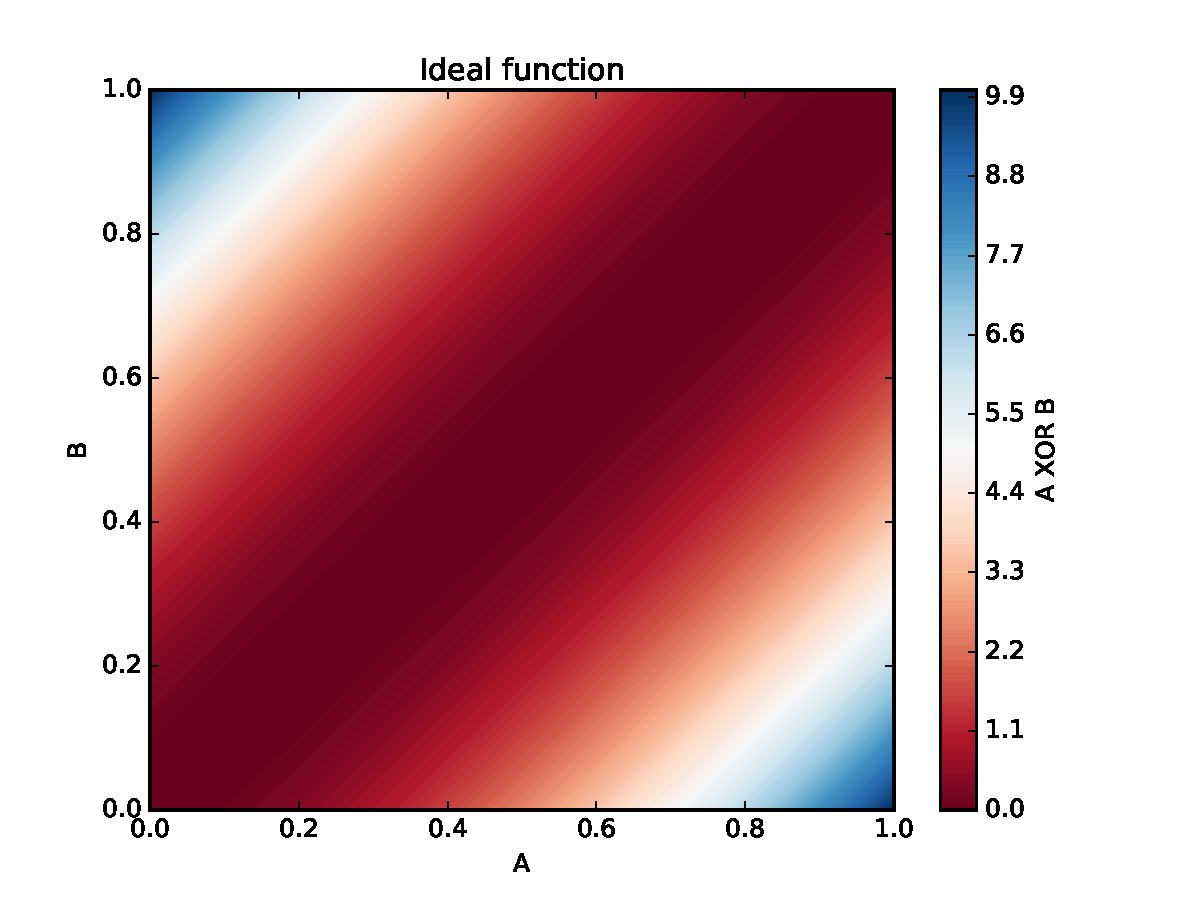
\includegraphics[width=0.6\textwidth]{IdealSurface.pdf} 
	\caption{Ideal continuous \textit{XOR} gate.}\label{fig:ideal}
\end{figure}
This modelling task evaluated the behaviour of the current system compared to the ideal behaviour shown in Figure (\ref{fig:ideal}). Additionally,  some parameters were tuned for a closer to ideal response. 
\newpage
\subsection{Chemical reactions}
The biological mechanism can be summarized by several small reactions. Those  reactions are occurring simultaneously. They provide the expected \textit{XOR} gate behaviour. The main steps are shown in Figure \ref{fig:steps}.
\begin{figure}[h]
	\centering
	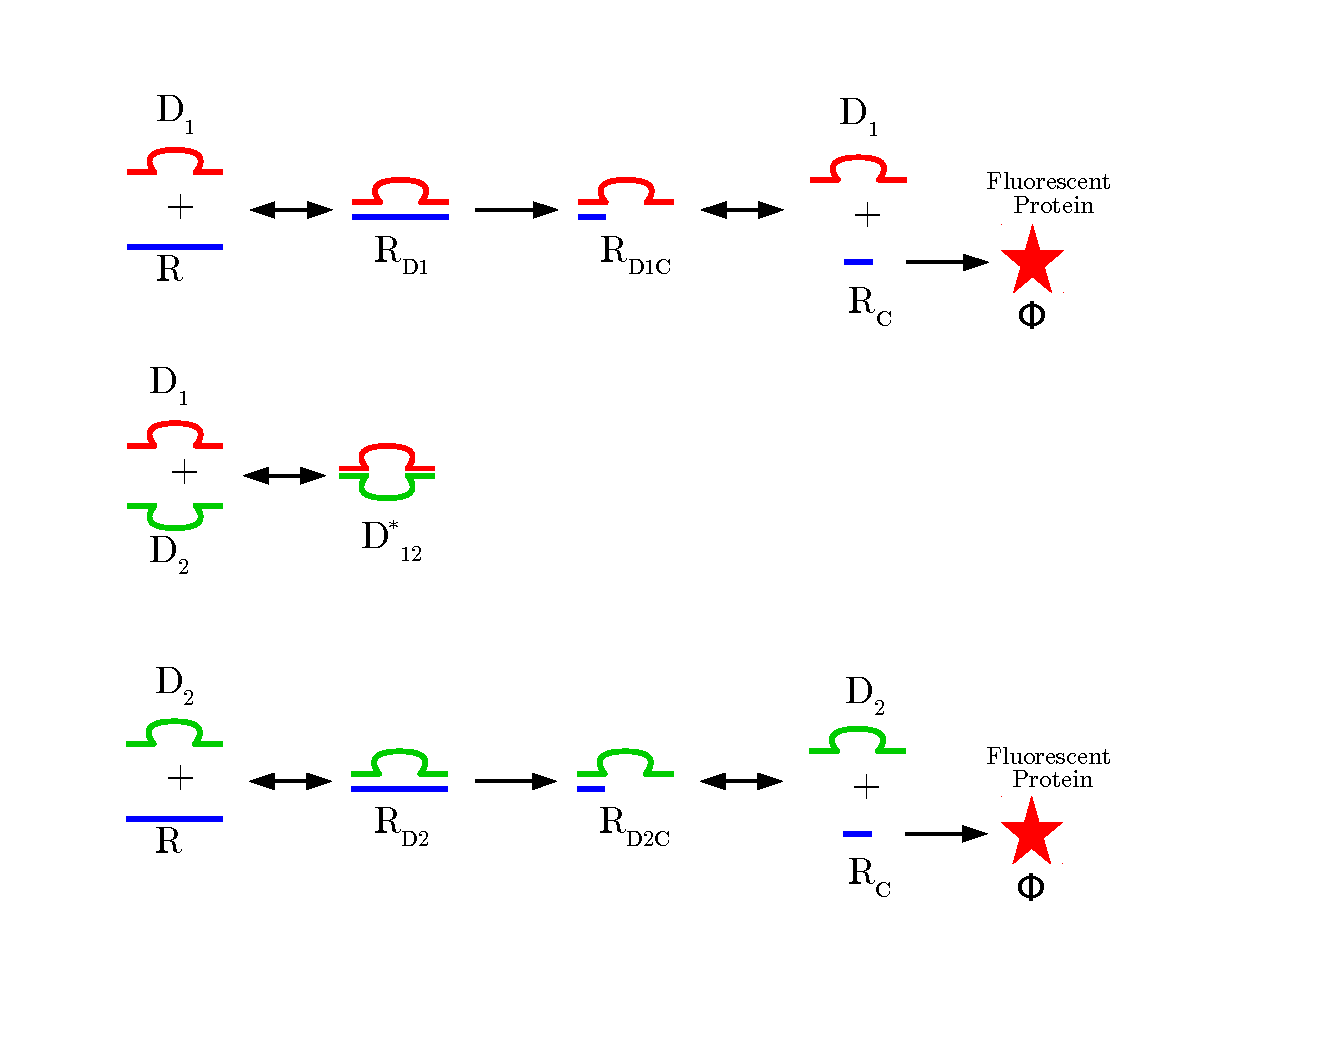
\includegraphics[width=0.6\textwidth]{ReactionSchematic.pdf} 
	\caption{Main chemical reactions.}\label{fig:steps}
\end{figure}\par 
It can be seen that when both species $D_1$ and $D_2$ are present, the production of fluorescent protein is inhibited. The model should consider all of these reactions happening simultaneously. Table \ref{tb:rxns} contains the information for all the relevant reactions and their kinetic constants.

\begin{table}[h]
	\centering
	\caption{Summary of modelled chemical reactions.} \label{tb:rxns}
	\begin{tabular}{c|c|c|c}
	Number & Reaction & $k[s^{-1}]$ & $K_{eq}$ \\ \hline 
	1 & $D_1+D_2 \rightleftharpoons D^*_{12}$ & $\num{5e-3}~$  & 1400  \\ 
	2 & $D_{1} + R \rightleftharpoons R_{D1}$ & $\num{5e-3}~$ & 10 \\ 
	3 & $D_{2} + R \rightleftharpoons R_{D2}$ & $\num{5e-3}~$ & 10 \\ 
	4 & $R_{D1} \rightarrow R_{D1C}$ & $\num{8.9e-3}~$ & - \\ 
	5 & $R_{D2} \rightarrow R_{D2C}$ & $\num{8.9e-3}~$ & - \\ 
	6 & $R_{D1C} \rightleftharpoons R_C + D_1$ & $\num{5e-1}~$ & 1000  \\ 
	7 & $R_{D2C} \rightleftharpoons R_C + D_2$ & $\num{5e-1}~$ & 1000 \\ 
	8 & $R_C \rightarrow R_c + \phi$ & $\num{1.5e-2}~$  & - \\ 
	9 & $D_1 \rightarrow \varnothing $& $\num{1e-3}~$ & - \\ 
	10 & $D_2 \rightarrow \varnothing$ & $\num{1e-3}~$ & - \\ 
	11 (Decay) & $i \rightarrow \varnothing $ & $\num{3.0e-3}~$  & - \\ 
	12 & $\phi \rightarrow \varnothing$ & $\num{3.9e-4}~$ & - \\ 
	13 & $R \rightarrow \varnothing$ & $\num{3e-3}~$ & - \\ 
	14 & $200 \rightarrow R$ & $\num{9.8e-2}~$ &-  \\ 
	15 & $U_1 \rightarrow D_1$ & $\num{9.8e-2}~$ & - \\ 
	16 & $U_1 \rightarrow D_1$ & $\num{9.8e-2}~$ & -
	\end{tabular} 
\end{table}
where: 
\begin{itemize}
 \item $i$ is $D^*_{12},R_{D1},R_{D2},R_{D1C},R_{D2C}$ and $R_{C}$.
 \item $U_1$ and $U_2$ are the promoters for the DNA chains ($D_1$ and $D_2$).
 \item $R^0$: This is the production parameter for the RNA sequence. This is a constant with value of 1.
\end{itemize}

The inverse reaction constant for a reaction \textit{i} is defined as: 
\begin{equation}
	q_i=\dfrac{k_i}{K_{i,eq}}
\end{equation}
\subsection{Differential equations}
The following are the different differential equations for each component present in the system: 
\begin{subequations}
	\begin{align}\label{eq:model}
	\frac{dD_1}{dt} &= -k_1D_1D_2+q_1D^*_{12}-k_2D_1R+q_2R_{D1}+k_6R_{D1C}-q_6R_cD_1-k_9D_1+k_{15}U_1\\
	\frac{dD_2}{dt} &= -k_1D_1D_2+q_2D^*_{12}-k_3D_2R+q_3R_{D2}+k_7R_{D2C}-q_7R_cD_2-k_{10}D_2+k_{16}U_2\\
	\frac{dR}{dt} &= -k_2D_1R+q_2R_{D1}-k_3D_2R+q_3R_{D2}-k_{13}+k_{14}R^0\\
	\frac{dR_{D1}}{dt} &= k_2D_1R-q_2R_{D1}-k_4R_{D1}-k_{11}R_{D1}\\
	\frac{dR_{D2}}{dt} &= k_3D_2R-q_3R_{D2}-k_5R_{D2}-k_{11}R_{D2}\\
	\frac{dR_{D1C}}{dt} &= k_4R_{D1}-k_6R_{D1C}+q_6R_cD_1-k_{11}R_{D1C}\\
	\frac{dR_{D2C}}{dt} &= k_5R_{D2}-k_7R_{D2C}+q_7R_cD_2-k_{11}R_{D1C}\\
	\frac{dR_C}{dt} &= k_6R_{D1C}-q_6R_CD_1+k_7R_{D2C}-q_7R_cD_2-k_{11}R_c\\
	\frac{d \phi}{dt} &= k_8R_C-K_{12}\phi \\
	\frac{dD^*_{12}}{dt} &= k_1D_1D_2-k_1D^*_{12}-k_{11}D^*_{12}
	\end{align}
\end{subequations}
\newpage
\section{Initial case}

\subsection{Dynamic simulation}
A dynamic simulation was carried out for this model. The following parameters were chosen:
\begin{itemize}
\item $U_1$ and $U_2$= 1. 
\item $R^0$=1.
\end{itemize}
Figure \ref{fig:dyn} shows that a steady state is achieved. There is a large concentration of pigment given that the inputs for both signals are present. 
\begin{figure}[h]
	\centering
	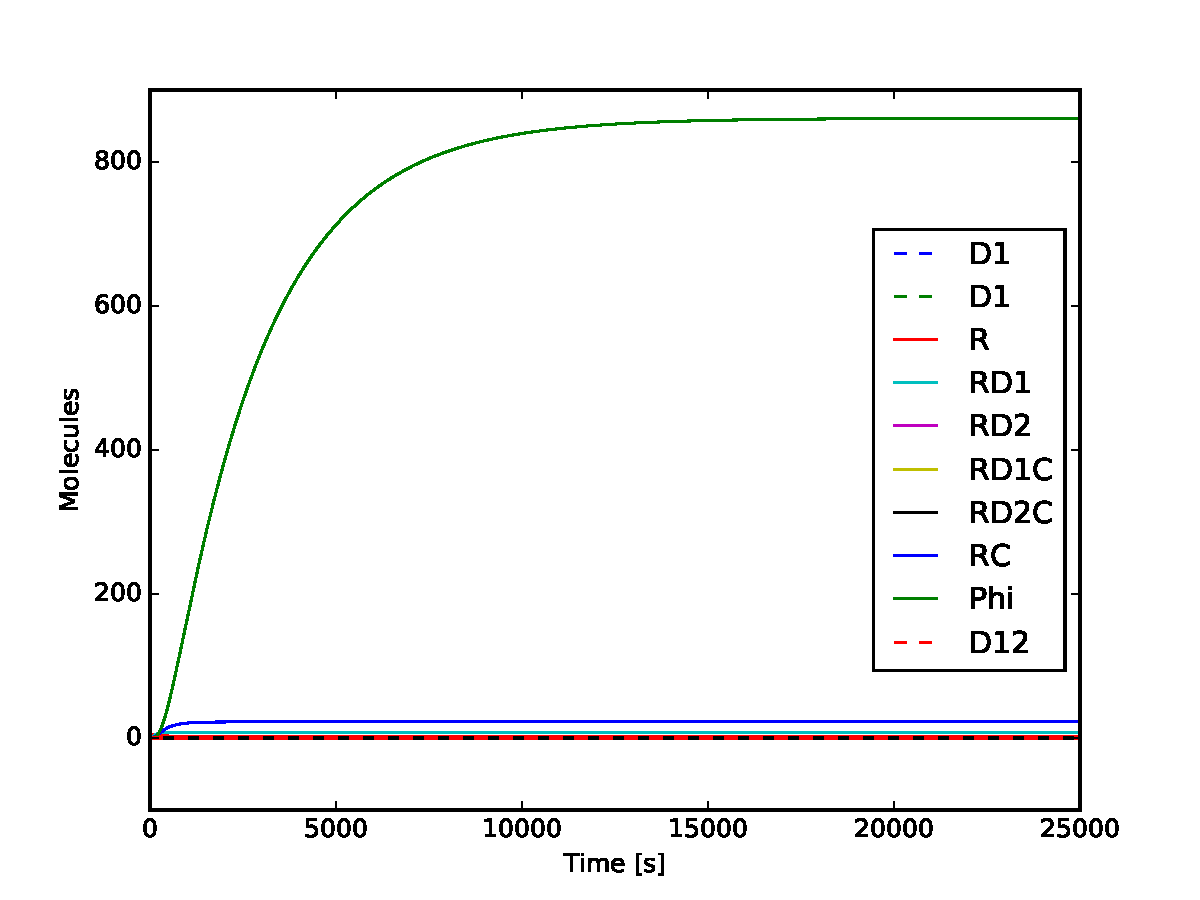
\includegraphics[width=0.6\textwidth]{Dynamic.pdf} 
	\caption{Dynamic response for the base case with inputs $U_1$ and $U_2$= 1.}\label{fig:dyn}
\end{figure}
 
\subsection{Surface response}
To carry out a comparison with the ideal response, it is necessary to evaluate the system in a given surface of points.\\
The selected ranges for the surface are: 
\begin{itemize}
\item $U_1~=~[0,1]$.
\item $U_2~=~[0,1]$
\item $R^0$=1.
\end{itemize}
The resulting surface is shown in Figure \ref{fig:surf}. 
\begin{figure}[h]
	\centering
	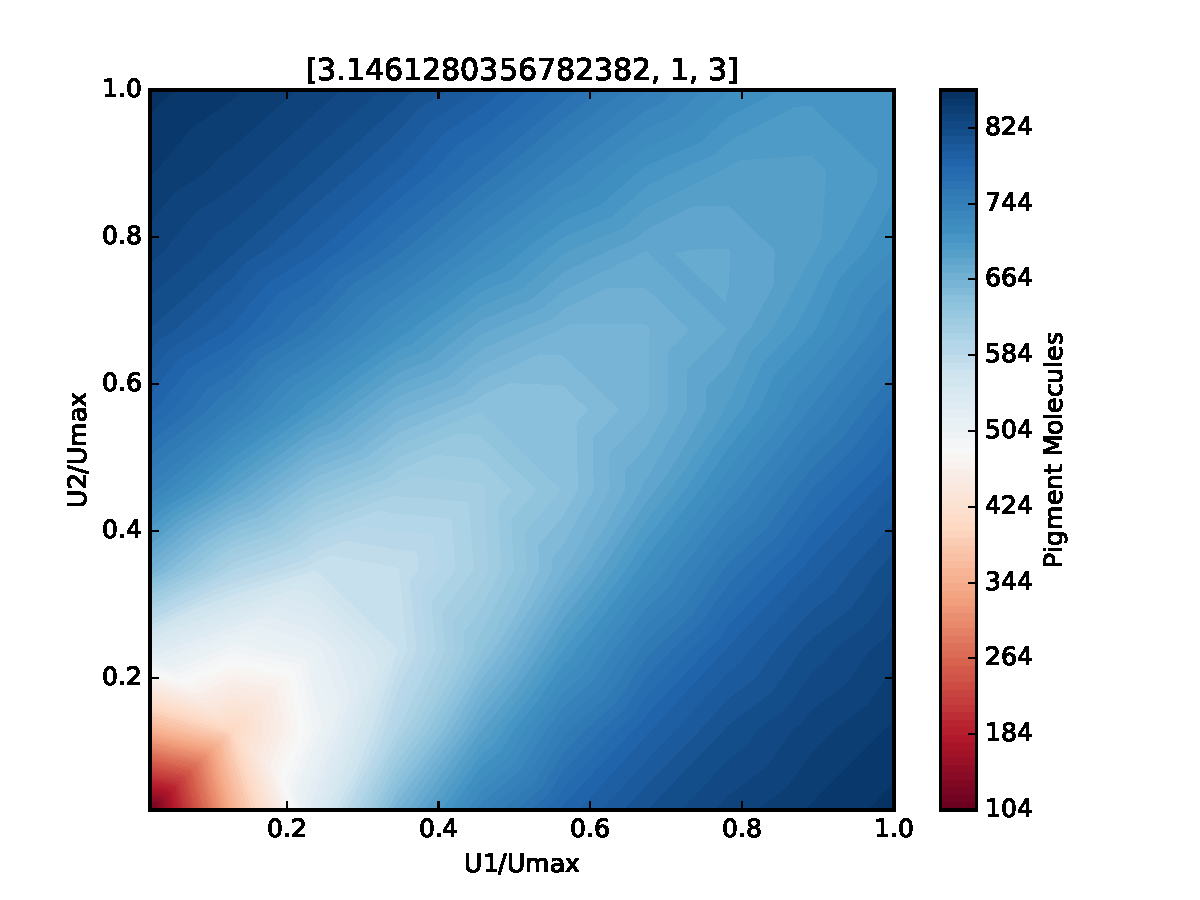
\includegraphics[width=0.6\textwidth]{Surface1.pdf} 
	\caption{Surface response for the base case with input range [0,1].}\label{fig:surf}
\end{figure}
\subsection{Observations}
Figure \ref{fig:surf} shows a trend that is similar to the ideal one. In the middle line ($U_1=U_2$) the values for the pigment concentration are considerably smaller compared to those in the corners. However, there is a very small difference when both inputs are close to the maximum. A careful use of the current system is recommended, in order to avoid a false positive due to high values of both inputs.
\newpage

\section{Improved case}
This result shows that there is still a possibility to make improvements in the system. These are done by modifying the values of the equilibrium constants as the DNA sequences $D_1$ and $D_2$ can be designed as well as some of the RNA ones.  
\subsection{Parameter tuning}
The constants required to be tuned are the following: 
\begin{itemize}
\item Reaction 1: $K_{1,eq}$.
\item Reaction 2,3: $K_{2,eq}$ Both reactions share the same equilibrium constant.
\item Reaction 6,7: $K_{6,eq}$ Both reactions share the same equilibrium constant.
\end{itemize}
The combinations were evaluated by two criteria: 
\begin{itemize}
\item \textit{Similarity to the ideal function.} This means that the trend should be as close as the ideal as possible. The situation where both components are present should be zero. 
\item \textit{Amount of pigment particles produced.} This ensures that the trend is kept for a significant amount of pigment particles. It is possible for some surface to have a behaviour close to ideal while producing very few pigment particles. 
\end{itemize}
The implementation of these two criteria into a single function for an optimization problem did not meet the requirements. Thus, a manual search over a space was carried out. The parameters where evaluated in a logarithmic scale. The following ranges were used: 
\begin{table}[h]
\centering
\caption{Equilibrium constants tuning ranges.} \label{tb:ranges}
\begin{tabular}{c|c|c}
Constant & Lower Bound & Upper Bound  \\ \hline
$K_{1,eq}$ & $10^{2}$  & $10^{6}$ \\ 
$K_{2,eq}$ & $10^{-4}$ & $10^{6}$  \\
$K_{6,eq}$ & $10^{-4}$ & $10^{6}$
\end{tabular} 
\end{table}

\subsection{Results}
Searching in the ranges summarized on Table \ref{tb:ranges}, the obtained values for the equilibrium constants are shown on Table \ref{tb:optcon}.
\begin{table}[h]
\centering
\caption{Final equilibrium constants values.} \label{tb:optcon}
\begin{tabular}{c|c}
Constant & Value \\ \hline
$K_{1,eq}$ & $10^{5}$  \\ 
$K_{2,eq}$ & $10^{-1.5}$ \\
$K_{6,eq}$ & $10^{3}$ 
\end{tabular} 
\end{table}
Figure \ref{fig:surfopt} illustrates the resulting surface. 
\begin{figure}[h]
	\centering
	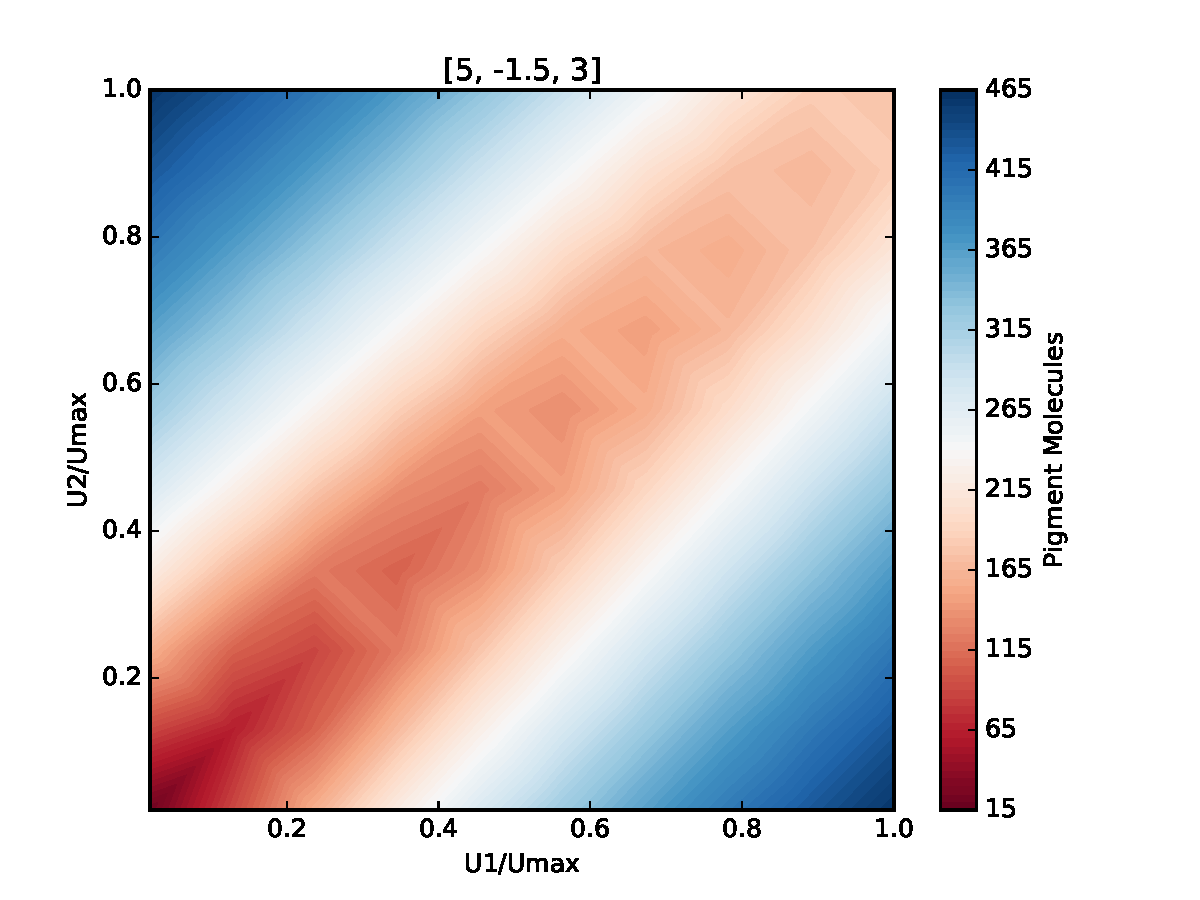
\includegraphics[width=0.6\textwidth]{Surface2.pdf} 
	\caption{Optimal surface response for the base case with input range [0,1].}\label{fig:surfopt}
\end{figure}
Figure \ref{fig:surfopt} shows a response very close to ideal. It has a very sharp difference for the case when there is only one input (between 350 and 465 pigment molecules) compared to the simultaneous inputs (15 to 165). Additionally, there is a significant amount of pigment molecules produced for when the gate response is positive (more than 300). \par 
The modifications on the constants have the following implications on the reactions: 
\begin{itemize}
\item $K_{1,eq}~ = ~10^{5}$. The component $D^*_{12}$ should be very stable and formed quickly. This ensures that the pigment production is inhibited while both molecules are present.
\item $K_{2,eq}~=~10^{-1.5}$. The first RNA binding (reactions 2 and 3)should be slow enough to allow both molecules $ D_1$ and $D_2$ to bind if they are present blocking the pigment production. If this reaction is too fast the inhibition reaction will not have a significant impact on the pigment production. 
\item $K_{6,eq}~=~10^{3}$. Reactions (6 and 7) should be fast. This allows for a quicker production of pigment and amplifies the effect from the previous equilibrium reactions.  
\end{itemize}
\section{Conclusions}\par
It was possible to model the \textit{XOR} logic gate system, both dynamically and steady state for a series of input.\par 
An expected response surface was computed and it shows a similar response to the ideal one using the current information.
\par 
The surface was improved by modifying the equilibrium constants in the model. This provided valuable feedback on the reactions that need to be promoted and those that need to be inhibited. 

\end{document}
